\paragraph{Energy intensities}
\note{include information about energy intensities}

\paragraph{Coefficient matrices}
\note{Add references about leontief matrix definition check references in \cite{Bartolucci2020}}
The economic coefficient matrix $A$ is used for the input-output analysis (IOA). Being $A$ an $n\times n$ matrix and $\mathbb{I}_n$ the identity matrix of dimension $n$. The Leontief inverse of $A$ is defined in equation \eqref{eq:leon}.
\begin{equation}
    L=\left(\mathbb{I}_n-A\right)^{-1}
    \label{eq:leon}
\end{equation}
for simplicity we will call $L$ the Leontief matrix and IA matrix to its inverse, $IA=\left(\mathbb{I}_n-A\right)=L^{-1}$. 

Being $A$ the economic coefficient matrix, $X$ the economic output and $FD$ the final demand, the equivalent relations in equations \eqref{eq:XFD} and \eqref{eq:FDX} can be defined, as $L=IA^{-1}=\left(\mathbb{I}_n-A\right)^{-1}$.
\begin{gather}
X=L\cdot FD\label{eq:XFD}\\
FD=IA\cdot X\label{eq:FDX}
\end{gather}

The economic coefficient matrix $A$ is provided in the inputs files. This matrix is assumed to be constant once the historic period is over. The matrix should be arranged as follows:
\begin{itemize}
    \item For the world model: it should be a matrix of sectors $\times$ sectors dimensions, as given in Figure \ref{fig:A0}.
\begin{figure}[H]
    \centering
    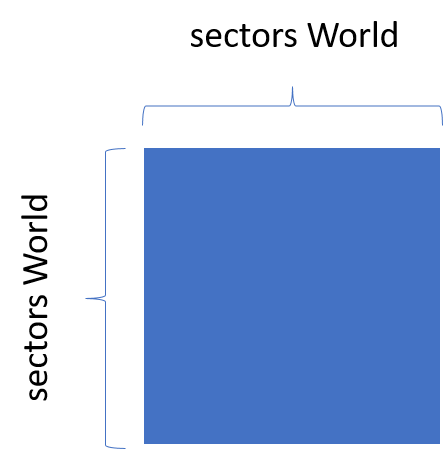
\includegraphics[scale=0.55]{figures/A0.png}
    \caption{Economic coefficients matrix for \modelsub{w} model.}
    \label{fig:A0}
\end{figure}
\item For a regional model: it should be a matrix of ($2\,\cdot$ sectors) $\times$ ($2\,\cdot$ sectors), where the first sectors block are the sectors of the region and the second block are the sectors of Rest of the World, see Figure \ref{fig:A1}.
\begin{figure}[H]
    \centering
    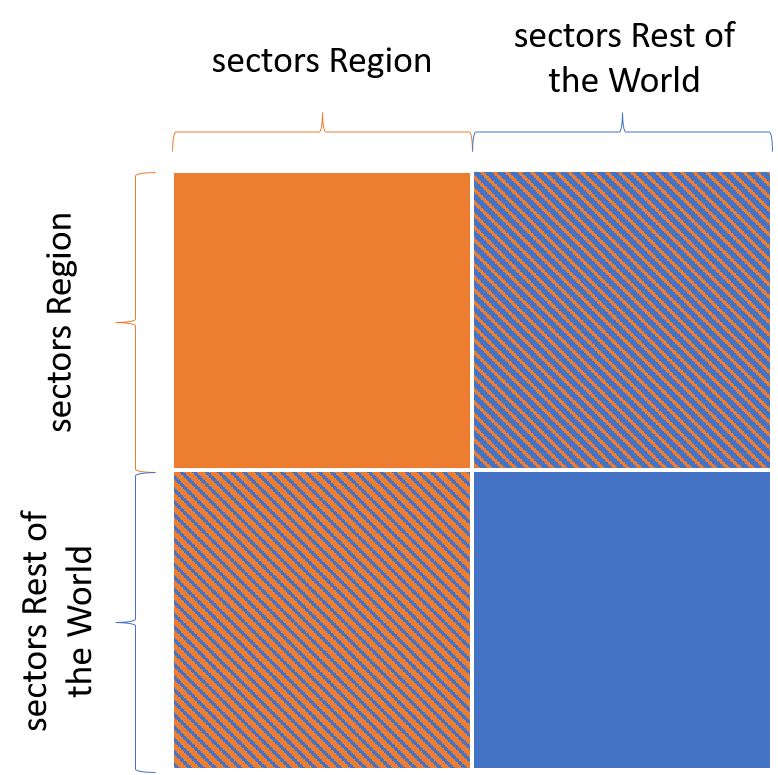
\includegraphics[scale=0.55]{figures/A1.png}
    \caption{Economic coefficients matrix for \modelsub{rg} model.}
    \label{fig:A1}
\end{figure}
\item For a subregional model: it should be a matrix of ($3\,\cdot$ sectors) $\times$ ($3\,\cdot$ sectors), where the first sectors block are the sectors of the subregion, the second block are the sectors of Rest of the Region, and the last block are the sectors of the Rest of the World. This representation is shown in Figure \ref{fig:A2}.
\begin{figure}[H]
    \centering
    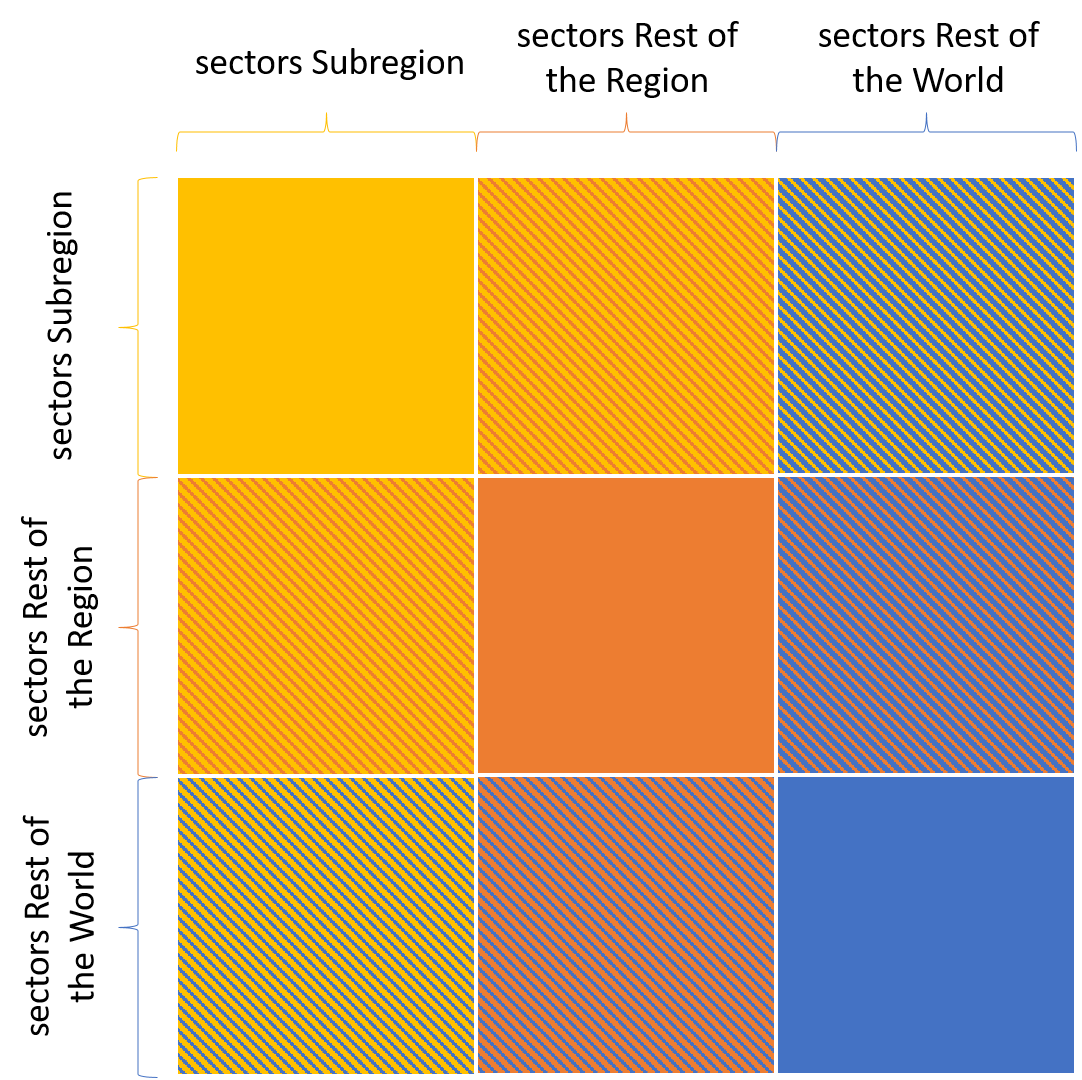
\includegraphics[scale=0.55]{figures/A2.png}
    \caption{Economic coefficients matrix for \modelsub{srg} model.}
    \label{fig:A2}
\end{figure}
\end{itemize}
\paragraph{Total outputs from demand}
\note{find a better way for this section}
Using the domestic final demand ($FD_D$) and the demand final demand of other regions ($FD_{RoX}$) the economic output ($OUT$) is computed.
\begin{equation}
    OUT=L_D\cdot FD_D+L_{exp,\,RoX}\cdot FD_{RoX}
\end{equation}
where $L_D$ is the domestic Leontief matrix, the full Leontief matrix in the world model and the upper-left submatrix of Leontief matrix in the regional and subregional models. $L_{exp,\,RoX}$ is the Leontief submatrix of exports to the Rest of Region X, $FD_{RoX}$ is the final demand of region X.
\note{continue}